\documentclass{beamer}
\usepackage[utf8]{inputenc}
\usetheme{Szeged}
\usecolortheme{beaver}
\usepackage[english]{babel}
\usepackage{ulem}
\usepackage{xmpmulti}
%Information to be included in the title page:
\title{Malayalam Text Recognition System}
\author{Aarya R. Shankar
			\and Amrith M
				 \and Anand R
					\and Sarathchandran S}
\institute{Department of Computer Science\and College of Engineering,Trivandrum}
\date{2015-2019}
 
\begin{document}

\frame{\titlepage}


\begin{frame}
\frametitle{Table of Contents:-}
\begin{itemize}
\item The Project
\item Our Work
\item Why we do this?
\item Existing Technology
\item How we do this?
\item Project Structure
\item Technology Stack
\item Conclusion
\end{itemize}

\end{frame}


\begin{frame}{What is it ?}

    \begin{columns}[c] % the "c" option specifies center vertical alignment
    \column{\textwidth} % column designated by a command
     Optical character recognition (also optical character reader, OCR) is the mechanical or electronic conversion of images of typed, 
handwritten or printed text into machine-encoded text, whether from a scanned document, a photo of a document, a scene-photo (for example the 
text on signs and billboards in a landscape photo) or from subtitle text superimposed on an image (for example from a television broadcast)
    \end{columns}
\end{frame}



\begin{frame}{What We Do?}
     We plan to develop an OCR system that reads printed or written Malayalam characters from images to text in an editable document form.
\end{frame}

\begin{frame}{Why We Do?}
     Currently many languages have an OCR dedicated to it, but we are yet to have an official OCR application for Malayalam.
\end{frame}

\begin{frame}{Existing Technology}
Lekha OCR by Space Kerala
\begin{itemize}
    \item Uses Hu Moments
    \item Uses SVM classifier
    \item Accuracy: 85 - 90 \%
\end{itemize}
\end{frame}

\begin{frame}
\frametitle{How We Do?}
This is the pipeline of what we plan to do as of now. 
 
\begin{itemize}
 \item\only<1>{Black Magic}\only<2->{\sout{Black Magic}}
 \item<2-> Deep Learning !!!
\end{itemize}
 
\end{frame}

\begin{frame}
\frametitle{Why Deep Learning ?}
\begin{itemize}
 \item<1->Deep learning is the fastest-growing field in machine learning. It uses many-layered Deep Neural Networks (DNNs) to learn levels of 
representation and abstraction that make sense of data such as images, sound, and text.
\end{itemize}
 
\end{frame}

 \begin{frame}{How We Do?}
     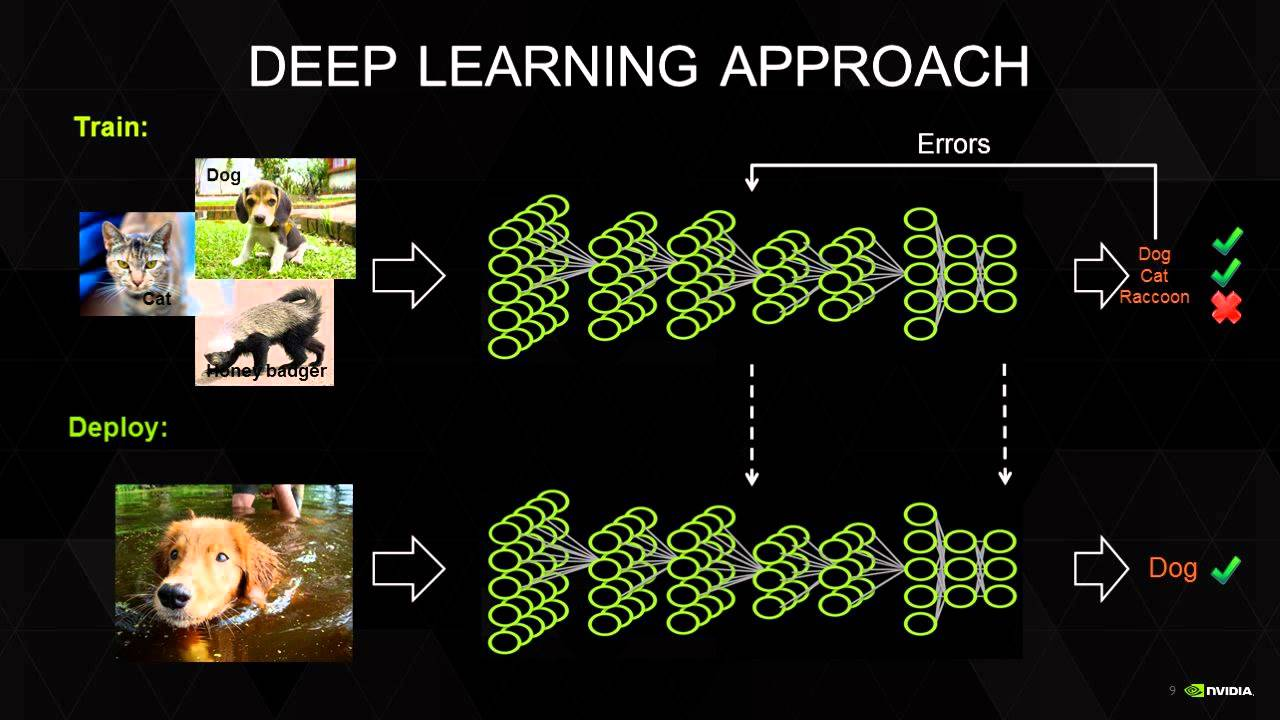
\includegraphics[height=7cm,width=\textwidth]{deep.jpg}
\end{frame}
 \begin{frame}{What We Use?}
 \textbf{Convolutional Neural Networks (CNNs)}
     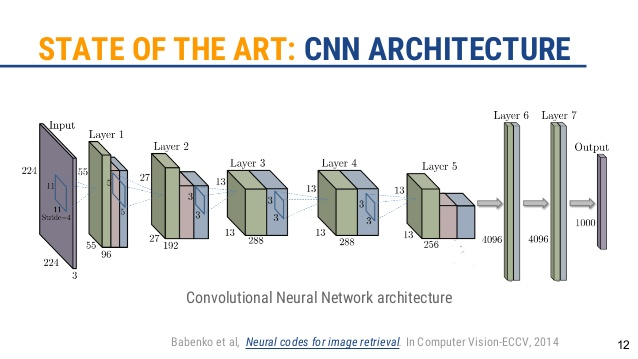
\includegraphics[height=6.5cm,width=\textwidth]{cnn.jpg}
\end{frame}

 \begin{frame}{What We Use?}
 \textbf{CNNs For Object Classification}
     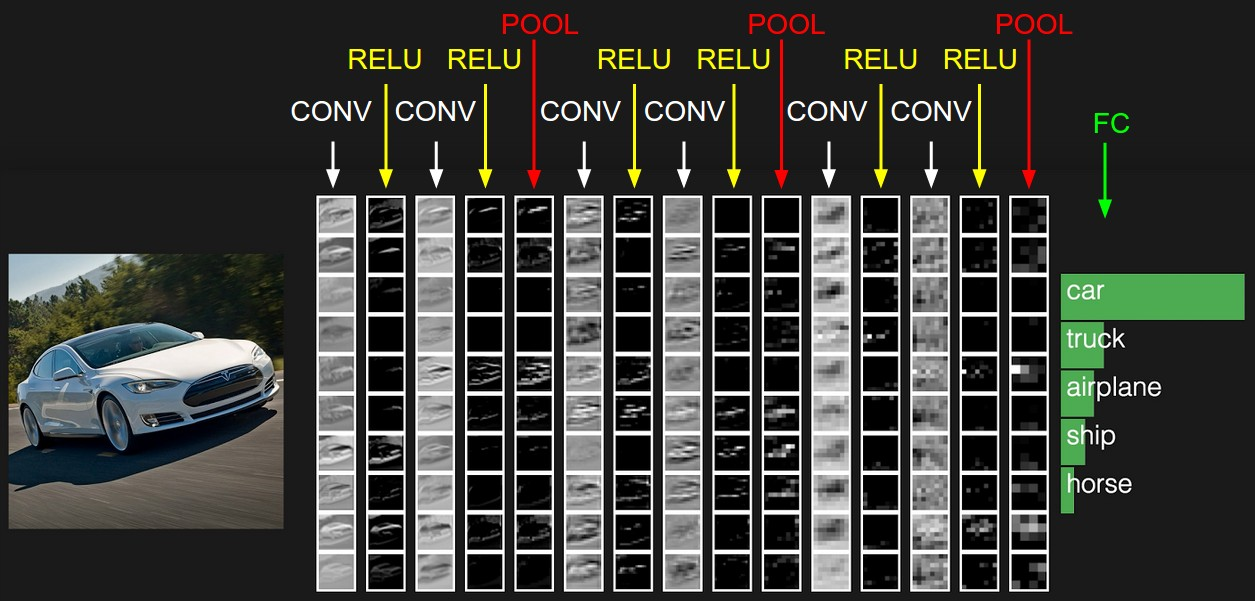
\includegraphics[height=6.5cm,width=\textwidth]{simpleconv.jpeg}
\end{frame}

\begin{frame}{The Image}
 \textbf{Convolutional Neural Networks (CNNs)}
     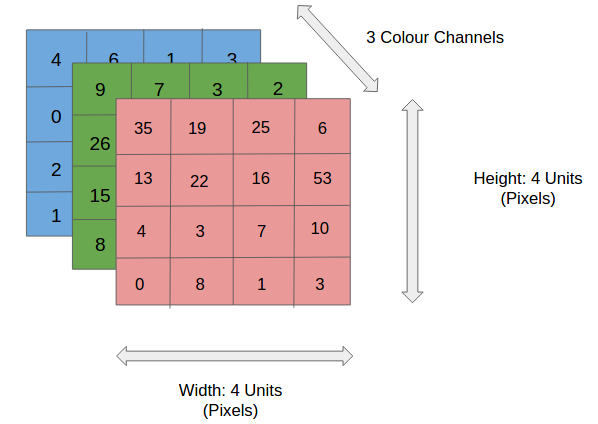
\includegraphics[height=6.5cm,width=\textwidth]{img.png}
\end{frame}

 \begin{frame}{Applying Convolution}
 \textbf{Convolutional Neural Networks (CNNs)}
    \transduration<0-8>{0}
        \multiinclude[<+->][format=png, graphics={width=\textwidth,height=6cm}]{conv}
\end{frame}

\begin{frame}
\frametitle{Why CNNs ?}
\begin{itemize}
\item<1->Convolutional Neural Networks (ConvNets or CNNs) are a category of Neural Networks that have proven very effective in areas such as image recognition and classification. ConvNets have been successful in identifying faces, objects and traffic signs apart from powering vision in robots and self driving cars.
 \item<2->ConvNets work because they exploit feature locality. They do it at different granularities, therefore being able to model hierarchically higher level features. They are translation invariant thanks to pooling units. They are not rotation-invariant per se, but they usually converge to filters that are rotated versions of the same filters, hence supporting rotated inputs.
\end{itemize}
\end{frame}

\begin{frame}
\frametitle{Project Structure}
\begin{itemize}
 \item<1->Preparing The DataSet
 \item<2->Learning With A CNN Architecture
 \item<3->Estimating Accuracy
 \item<4->Tuning the parameters
 \item<5->Deploying the Model

\end{itemize}
\end{frame}

\begin{frame}{Technology Stack}
 \setbeamertemplate{itemize items}[ball]
 \begin{itemize}
  \item Python
  \item Keras
  \item Jupyter-Notebook
  \item Matplotlib
  \item GPU

  \end{itemize}
\end{frame}

\begin{frame}{Conclusion}
 \setbeamertemplate{itemize items}[ball]
 We hope to develop an open source deep learning model for Malayalam OCR.
\end{frame}

\end{document}


